\section{Related Work}



%Theories of sense of agency + example
The most widely used theory on the sense of agency is the comparator model. It states that our brain when we perform a voluntary, intentional action, generates a sensory prediction, which is compared to the actual sensory feedback received from the sensory system. If the comparison reveals no sensorimotor incongruency, a sense of agency arises (sources). Imagine pressing the key of a piano to produce a tone. In such simple interaction, it is unequivocally clear that we are the ones performing the movement and causing the tone. We experience authorship. 

This straightforward relationship is complicated by the introduction of technology. Think about, playing a computer game where a key press controls an avatar playing the piano. Here, we do not really press the piano key, the avatar's movement, and the tone are now generated by a computer. Despite the blurring lines between the performer and the cause of the tone, we still feel a sense of authorship when the comparison does not reveal incongruency. This lingering feeling of control is thought to be elicited by our intentions being reflected in the resulting action (sources needed). 

In situations without intentional action, our brain does not generate predictions. Thus, in alignment with the cooperator model, researchers generally measured a lower sense of agency when actions were externally triggered (e.g., by brain simulation (Haggard and Clark, 2002), the body part being moved by another person (Kühn 2013). Accordingly, playing a tune on a piano with technology causes our figure movement, our body performs the action but we do not have the intention to play. We will most likely will lack a sense of agency.



However, action augmentation technology using motor actuation aims to augment the user’s actions diminishing the SoA (see Cornelio 2022). 



%old
- %intro
In a simplified world, intentional movements directly leading to external events provide a strong sense of responsibility and control over the action's outcome. For instance, when we press a piano key, it is unequivocally clear that we are the ones performing the movement and causing the tone. However, the introduction of technology can complicate this relationship. Imagine playing a computer game where a key press controls an avatar playing the piano. The avatar's movement is now generated by a computer, blurring the lines between the performer and the cause of the tone. Despite this complexity, research (sources to be provided, such as wn and Imamizu) suggests that as long as the button press and the avatar's movement remain consistent, we still feel a sense of authorship over the tone as a consequence of our action. This lingering sense of control might be due to our intentions being reflected in the resulting action (sources needed). 

In augmented interactions, the dynamics change. When technology moves our fingers, our body performs the action, but we may experience a diminished feeling of causing the action [sources - augmented actions lead to less agency; check Yoshi und Harrard 2013, Moore, Wegner und Harrard 2009, Haggard, Clark 2002]. 

- no intentional binding when action is triggerd by brain stimulation  (Haggard, P., Clark, S. & Kalogeras, J. Voluntary action and conscious awareness. Nat. Neurosci. 5, 382–385 (2002).
- 
The feeling of agency seems to be 

However, now  Imagine playing a computer game where a key press controls an avatar playing the piano. The avatar's movement is now generated by a computer, blurring the lines between the performer and the cause of the tone. Despite this complexity, research (sources to be provided, such as wn and Imamizu) suggests that as long as the button press and the avatar's movement remain consistent, we still feel a sense of authorship over the tone as a consequence of our action.


%old 
A sense of agency is the feeling of intentional actions and their external consequences (Haggard, 2017).
It is implicitly explained within the framework of motor control (see Frith and collegus 2000). When we perform an action without any external interference, the sensory consequences of that action align with the predicted sensory consequences, which are based on a copy of motor commands (i.e., efference copy). However, in situations where the movement is elicited by an external cause, as in augmented actions, the predicted sensory consequences may differ or be absent altogether. In such cases, the actual sensory feedback does not match the predicted sensory feedback. 

According to this account, the feeling of agency arises only when the predicted sensory feedback perfectly corresponds to the actual sensory feedback. In other words, when our actions and their outcomes align seamlessly, we experience a sense of agency over those actions (see figure \ref{fig:com_model}. 



\begin{figure}
    \centering
    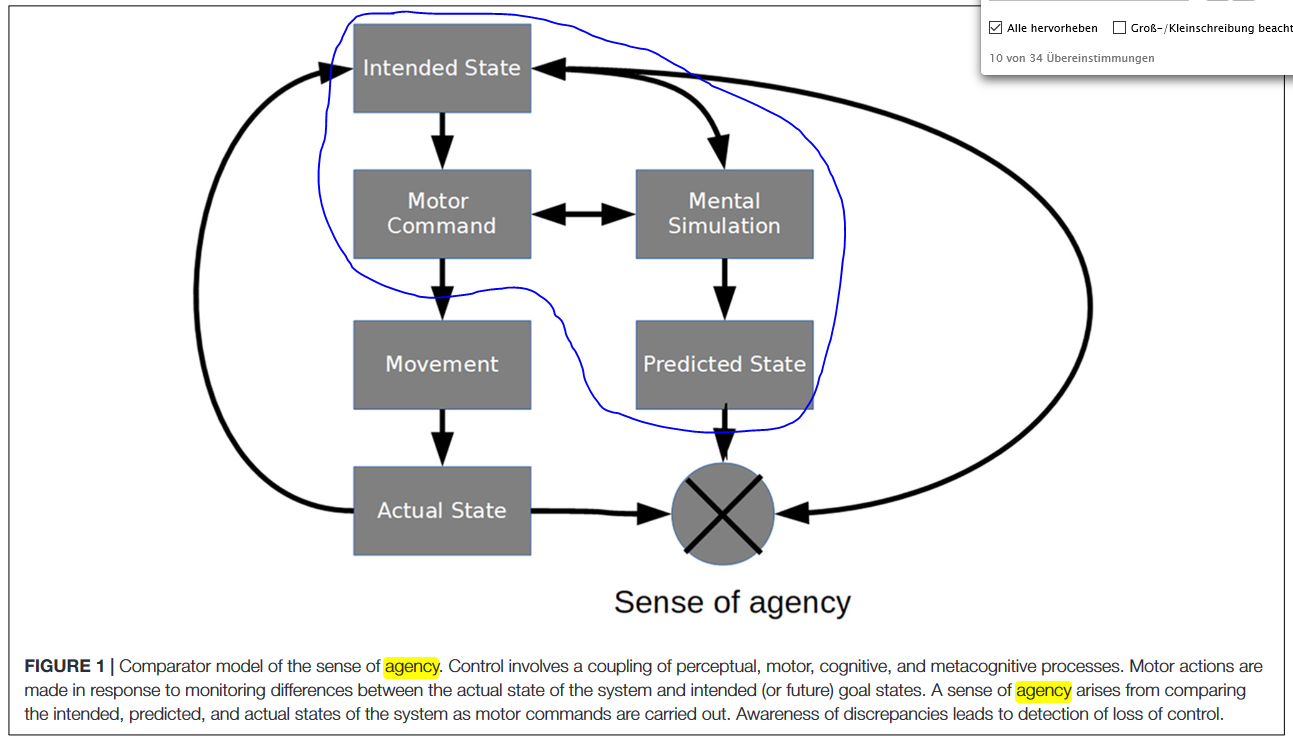
\includegraphics[width=\columnwidth]{figures/augmented_com_model_draft.png}
    \caption{draft - visualization of comparator model of the sense of agency in the case of augmented interactions (inspired by Dewey 2019)}
    \label{fig:com_model}
\end{figure}
(see Carruthers 2012 for a summary of arguments against this model)

% relevance of sense of agency
- motor learning ( check Wen, W. et al. Perception and control: individual difference in the sense of agency is associated with learnability in sensorimotor adaptation. Sci. Rep. 11 , 20542 (2021).)

% In this paper, we present a physical action augmentation prototype and a user study to investigate the experience of agency during the use of the prototype. Hence, our research builds on previous qualitative and quantitative research on the sense of agency.
% on actuated haptic systems, brain-computer interfacing as well as
% moving the finger of a user when the user intends to do so, but before the user directs their muscles to move.

%Our research builds on previous engineering work in brain-computer interfacing and on theories of the sense of agency as discussed in cognitive science and neuroscience.


\subsection{The sense of agency in human-computer interaction}
% LT to write first version
\begin{comment}


% Sense of agency in augmented interaction 

- intention / voluntary movement is important for sense of agency
- involuntary movements produce less binding than do voluntary actions, or even reverse the effect entirely (Yoshi und Harrard 2013, Moore, Wegner und Harrard 2009)
it has been shown, that mere peripheral body movements, elicited by TMS simulations, produce a perceptual repulsion opposite to intentional binding in truly operant intentional actions (Haggard, Clark 2002)

There is an ongoing debate, whether the temporal attraction is specific to intentional movements, or is more generally related to the perception between action and outcome (Buhner 2012)
--> they suggest intentional action is not necessary for temporal binding, but that the binding results from a causal relation linking actions with consequences -- more general causal binding -- do we need to go there?

One idea: - reach "we-mode" in human-machine joint control ---> decode human intention (Zander 2011, Felke 2019, Shiskin 2016)
- maintain sense of agency in augmented interactions 
- doing this by leveraging action intention in brain



Experiencing control is an important factor in human-computer interaction (see Shneiderman and Nielsen). 

%%%%%%%%%% theory on sense of agency  / neural basis of sense of agency

The sense of agency, or this being in the "driving seat when it comes to our own actions"~\cite{Moore2016-ub} can be subdivided into the \textit{feeling} of agency, a low-level pre-reflective sensory process, and the \textit{judgement} of agency, a higher level reflective cognitive process, ~\cite{Moore2016-ub, Danry2022-xk}.

Agency is largely explained with a comparator model, describing internal computational mechanisms of human action control 
-- comparator model (Blakemore 2002, Frith 2000, Frith 2005)
-- integrate predictive coding??

- In the words of Harrard: making an association between action and outcome (Intention - Volition-Movement-Agency -Effect) --> find the source; is from yt video

- Looking at the sense of agency from the perspective of the comparator model
    - if prediction and sensory feedback match = we perceive sense of agency - not only for the big loop with sensory feedback (beep), but also for the forward loop (smaller) --> I can still think that I turned the light on, even if it takes 10 sec after pushing the switch, cause movement still worked as predicted

- In Augmented movements different (explain)
- Before deep diving in these results - excurse on how to measure agency

\subsection{Measuring agency experience}



% explicit measures - reflective (short paragraph)
% - questionnaires

%% from bergström 22
- read 18, 37 from  Bergstöem 
- 14,14,19.31,39,41,48
11,20,33

Sense of control is mostly measured with simple items with ratings like "It felt like I was in control of the hand I was looking at” rated on a 7-point Likert scale, +3 indicating strong agreement and −3 indicating strong disagreement (Longo and Haggard) or  "Indicate how much it felt like moving the joystick caused the object on the computer screen to move” as a measure of explicit sense of agency, also rated on a 7-point scale" (11) 
item asking participants to indicate the degree of control they have felt over the changes on the screen [1]. We used this item also as an agency measure (1) 

Researchers use implicit and explicit methods. Explicit methods involve directly asking participants to report their subjective experiences using items rated on Likert scales or percentages. These items, such as "It felt like I was in control of the hand I was looking at" (Longo & Haggard) and "Indicate how much it felt like moving the joystick caused the object on the computer screen to move" (Ebert & Wegner), may focus on either the action element or the outcome element of the sense of agency (see Moore).



( van der Wel et al., 2012; Chambon et al., 2013),“ 
Individuals’ sense of agency can be estimated with explicit self-reported measures using Likert’s scales or percentages ( van der Wel et al., 2012; Chambon et al., 2013),“ 

Items such as ""It felt like I was in control of the hand I was looking at” (longo Haggard) and "Indicate how much it felt like moving the joystick caused the object on the computer screen to move” (Ebert und Wegner). Notably, such items differ between focusing either on the action element or the outcome element (See MOore)



% - phenomenological interview

% implicit measures - pre-reflective (longer paragraph)
-subjective measures address a high level-SoA  based on subjective judgments of feeling of control (Barlas and Kopp)
- proxy for the low-level SoA as they do not require conscious reflection on one’s SoA (Synofzik et al., 2008a; Desantis et al., 2011; Moore and Obhi, 2012; Barlas and Obhi, 2014).“ ([Barlas und Kopp, 2018, p. 2]
- one such measure is intentional binding

% - intentional binding: explain what this is and give a bit more detail about the underlying mechanisms and ideas about whats going on in the brain here
- „refers to the perceived temporal attraction between voluntary actions and their outcomes (Haggard et al., 2002). More clearly, the temporal interval between actions and outcomes is perceived as shorter when these outcomes are produced by voluntary actions compared to when they follow, for instance, involuntary movements or external causes (Haggard et al., 2002).“ ([Barlas und Kopp, 2018, p. 2]
- While details about the relationship between measures of intentional binding and SoA are far from clear, they are extensivly used 
- alternatives to intentional binding - sensory attenuation / visual attention




\textit{Intentional binding} is the phenomenon of subjectively compressing the time interval between a voluntary action and the sensory consequences of that action~\cite{Moore2012-ic}.
- comparisons between active and passive finger tab 
    Kühn 2013 + Engbert 2007 : experimenter presses the finger down in a passive condition
    
    
When a voluntary action is causally linked with a sensory outcome, the action and its consequent effect are perceived as being closer together in time. This effect is called intentional binding.“ (from Jo 2014)

- Read More 2009 (interval estimations were shorter (i.e., stronger binding) in voluntary than involuntary movements) 
- add figuure action binding and effect binding (e.g.  in WEN and Imamizu)


!! new paper suggesting that temporal binding / intentional binding is not a measure of sense of agency !!(Gutzeit!)  


% connection between implicit and explicit measures

- intentional binding effects are sometimes discrepant from explicit judgment of agency (see 30-33 in Wen and Imamizu) (Saito 2015; Majchrowitz 2018; Ebert
- Intentional binding is e.g. influenced by causal relations between events, attention, and arousal (see Wen and Imamizu)



% Sense of agency in augmented interaction 

- intention / voluntary movement is important for sense of agency
- involuntary movements produce less binding than do voluntary actions, or even reverse the effect entirely (Yoshi und Harrard 2013, Moore, Wegner und Harrard 2009)
it has been shown, that mere peripheral body movements, elicited by TMS simulations, produce a perceptual repulsion opposite to intentional binding in truly operant intentional actions (Haggard, Clark 2002)

There is an ongoing debate, whether the temporal attraction is specific to intentional movements, or is more generally related to the perception between action and outcome (Buhner 2012)
--> they suggest intentional action is not necessary for temporal binding, but that the binding results from a causal relation linking actions with consequences -- more general causal binding -- do we need to go there?

One idea: - reach "we-mode" in human-machine joint control ---> decode human intention (Zander 2011, Felke 2019, Shiskin 2016)
- maintain sense of agency in augmented interactions 
- doing this by leveraging action intention in brain




% RESEARCH GAP




\subsection{Sense of agency and actuated haptic systems}


\ subsection{Movement Intention}
idea: when we now compare completely voluntary movements with movements triggerd by the brain signal of our intention to move - what happens?

% close this paragraph with the problem that of the control mechanism of the actuator hardware and the disruotion in agency

% PosssessedHand, Gilbert-I miss being me, 


%%%%%%%%%%%%%%%%%%%%%%
Other
- EEG patterns related to readiness potential and intentional  binding sometimes show disceprant patterns ( see WEN and Imamizu 38 und 39) (wittmann 2014, Goldberg 2017)
\end{comment}